\documentclass{article}
\usepackage[utf8]{inputenc}
\usepackage[margin=2cm]{geometry}
\usepackage{amsmath}
\usepackage{amssymb}
\usepackage{amsthm}
\usepackage{graphicx}
\usepackage{subfig}
\usepackage{enumitem}

\usepackage{algorithm}
\usepackage{algorithmicx}
\usepackage{algpseudocode}

\usepackage{tikz}
\usetikzlibrary{positioning}

\title{Conditional SMC genealogies}
\author{Suzie Brown\\ {\small supervised by Adam Johansen, Jere Koskela, Paul Jenkins \& Dario Span\`o}}
\date{6 June 2018}

%\usepackage[colorlinks=true, allcolors=blue]{hyperref}
\usepackage[round, sort&compress]{natbib}
\usepackage{har2nat} %%% Harvard reference style
\bibliographystyle{agsm}

\newcommand{\E}{\mathbb{E}}
\newcommand{\PR}{\mathbb{P}}
\newcommand{\V}{\operatorname{Var}}
\newcommand{\vt}[2][t]{v_{#1}^{(#2)}}
\newcommand{\vttilde}[2][t]{\tilde{v}_{#1}^{(#2)}}
\newcommand{\wt}[2][t]{w_{#1}^{(#2)}}
\newcommand{\eqdist}{\overset{d}{=}}
\newcommand{\Bin}{\operatorname{Bin}}
\newcommand{\N}{\mathcal{N}}
\newtheorem{thm}{Theorem}

\begin{document}
\maketitle

\section{Introduction}
Sequential Monte Carlo has become a popular tool, particularly in applications such as object tracking, where there is a natural sequential component and we wish to infer underlying states from noisy observations.
While particle methods can be very effective for filtering, it is more difficult to apply them to smoothing because they typically suffer very badly from ancestral degeneracy in the particle genealogies.

When attempting to mitigate this problem, one often encounters a trade-off between ancestral degeneracy (arising from resampling) and weight degeneracy (arising from sequential importance sampling). However, while weight degeneracy is a reasonably well-quantified problem, there exists little in the way of tools for quantifying ancestral degeneracy a priori. There have been some simulation studies attempting to cast light on the magnitude of this problem, but analytical findings remain elusive, since the complexity of the most commonly used particle methods makes it difficult to obtain any rigorous results.
Consequently, there is a wealth of pertinent open questions in this area. This work attempts to extend a first result for a standard class of SMC algorithms to the case of conditional SMC with multinomial resampling. We hope this will serve as a first step towards analysing the more complex conditional SMC algorithms that are widely used in practice, particularly within the popular particle Gibbs algorithm.

This work exists at the interface of sequential Monte Carlo methods and population genetics, and the relevant material from each field is summarised in Sections \ref{sec:smc} and \ref{sec:popgen} respectively. 
Section \ref{sec:previous} summarises some known results about asymptotic genealogies, both with reference to population models and particle systems.
Section \ref{sec:theory} presents the theoretical aspect of our contribution, which is complemented by a simulation study in Section \ref{sec:simulations}.

\section{Background}
\subsection{Sequential Monte Carlo}\label{sec:smc}
References for this section are \citet{doucet2001}, \citet{delmoral2006}, and \citet{doucet2009}.

Although sequential Monte Carlo (SMC) methods can be applied in a much more general setting, they are particularly easy to motivate in the setting of state space models, where the ``sequential'' nature follows naturally from the discrete time steps present in the model. 
For the purposes of presenting the algorithm, let us consider a generic hidden Markov model (HMM) with hidden states $X_{0:M}$ and observables $Y_{0:M}$. We assume for notational convenience that $x_0,\dots,x_M$ take values in a common state space $\mathcal{X}$, and $y_0,\dots,y_M$ in a common state space $\mathcal{Y}$, although these assumption may be dropped. 
We make extensive use of the concise notation $z_{r:s} := \{z_r, z_{r+1}, \dots, z_s\}$.
Consider the HMM specified as follows.
\begin{align*}
& X_0 \sim \mu(\cdot) \\
& X_{t+1} \mid (X_t = x_t) \sim f(\cdot \mid x_t)  \qquad t=0,\dots,M-1 \\
& Y_t \mid (X_t = x_t) \sim g(\cdot \mid x_t) \qquad t=0,\dots,M
\end{align*}
with the conditional independence structure
\begin{align*}
& X_{t+1} \perp X_{0:t-1}, X_{t+2:M} \mid X_t \\
& Y_t \perp Y_{0:t-1}, Y_{t+1:M}, X_{0:t-1}, X_{t+1:M} \mid X_t
\end{align*}
for all $t$, as represented graphically below.

\begin{center}
\begin{tikzpicture}
\node (yt) {$Y_t$};
\node (thet) [below=of yt] {$X_t$};
\node (yt1) [left=of yt] {$Y_{t-1}$};
\node (thet1) [below=of yt1] {$X_{t-1}$};
\node (dot1) [left=of thet1] {$\dots$};
\node (dot2) [right=of thet] {$\dots$};
\draw[->](thet.north)--(yt.south);
\draw[->](thet1.north)--(yt1.south);
\draw[->](thet1.east)--(thet.west);
\draw[->](dot1.east)--(thet1.west);
\draw[->](thet.east)--(dot2.west);
\end{tikzpicture}
\end{center}

The conditional independence structure implies that the (joint) marginal distribution of the hidden states $X_{0:t}$ is given by
\begin{equation*} \label{eq:hmm_marginal}
p(x_{0:t}) = \mu(x_0) \prod_{i=1}^t f(x_i \mid x_{i-1})
\end{equation*}
and that the likelihood of the observations $y_{0:t}$ given the underlying states $x_{0:t}$ takes the form
\begin{equation*} \label{eq:hmm_likelihood}
p(y_{0:t} \mid x_{0:t}) = \prod_{i=0}^t g(y_i \mid x_i).
\end{equation*}

There are three main inference problems of interest in HMMs, namely: estimating the filtering distributions $p(x_t \mid y_{0:t})$, smoothing distributions $p(x_{t} \mid y_{0:M})$ and predictive distributions $p(x_{t+1} \mid y_{0:t})$. 
The smoothing distribution $p(x_{t} \mid y_{0:M})$ is obtained from $p(x_{0:M} \mid y_{0:M})$ by marignalising. Using the conditional independence structure, we can write
\begin{align}
p(x_{0:t} \mid y_{0:t}) &\propto g(y_t \mid x_t) f(x_t\mid x_{t-1}) p(x_{0:t-1}\mid y_{0:t-1}) \label{eq:smooth_recursion}\\
&\propto \mu(x_0) g(y_0\mid x_0) \prod_{i=1}^t f(x_i \mid x_{i-1}) g(y_i\mid x_i) \label{eq:smooth_recursion2}
\end{align}
for $t = 0,\dots,M$, where the one-step recursion \eqref{eq:smooth_recursion} is obtained using Bayes rule, and \eqref{eq:smooth_recursion2} is obtained by applying \eqref{eq:smooth_recursion} $t$ times. 
The filtering distribution $p(x_t \mid y_{0:t})$ can be obtained from \eqref{eq:smooth_recursion} by marginalising out $x_{0:t-1}$, which is straightforward if a Monte Carlo approximation is available.
The predictive distributions can also be derived from the smoothing distributions using
\begin{equation*}
p(x_{t+1}\mid y_{0:t}) = g(x_{t+1} \mid x_t) p(x_{0:t} \mid y_{0:t}).
\end{equation*}

SMC provides a method to approximate to \eqref{eq:smooth_recursion}, given a model specification and a sequence of observations. Like the underlying process, the algorithm proceeds sequentially, returning its approximation to the smoothing distribution at each time step.
A generic SMC algorithm is presented below.
\begin{algorithm}
	\caption{Standard SMC}\label{alg:SMC}
	\begin{algorithmic}[0]
    	\State \textbf{Inputs:} $\mu:\mathcal{X}\to[0,1];\quad f:\mathcal{X}\times\mathcal{X}\to[0,1];\quad g:\mathcal{Y}\times\mathcal{X}\to[0,1];\quad y_{0:M}\in\mathcal{Y}^M;\quad N\in\mathbb{N}$
		\For{$i = 1,\dots,N$}		
			\State $x_0^{(i)} \sim \mu(\cdot)$ \Comment initialise
			\State $\tilde{w}_0^{(i)} \gets g(y_0 \mid x_0^{(i)})$
			\State $w_0^{(i)} \gets \tilde{w}_0^{(i)} / \sum \tilde{w}_0^{(j)}$
		\EndFor
		\For{$t=1,\dots,M$}
        	\For{$i = 1,\dots,N$}
        		\State $\tilde{x}_t^{(i)} \gets$ {\footnotesize RESAMPLE}($\mathbf{x}_{t-1}, \mathbf{w}_{t-1}$) \Comment resample particles
				\State $x_t^{(i)} \sim f(\cdot \mid \tilde{x}_t^{(i)})$ \Comment propagate particles
				\State $\tilde{w}_t^{(i)} \gets g(y_t \mid x_t^{(i)})$ \Comment calculate weights
				\State $w_t^{(i)} \gets \tilde{w}_t^{(i)} / \sum \tilde{w}_t^{(j)}$ \Comment normalise weights
        	\EndFor
        \EndFor
	\end{algorithmic}
\end{algorithm}

There is a great deal of flexibility in the function referred to as {\footnotesize RESAMPLE} in Algorithm \ref{alg:SMC}. The most basic choice is multinomial resampling \citep{efron1994}, but it is far from optimal in terms of estimation variance \citep{douc2005}. Various alternative choices for the {\footnotesize RESAMPLE} function have been suggested in attempts to improve the algorithm's performance, some of which we discuss later.

If only the filtering distribution is required, we can marginalise out $\mathbf{x}_{0:t-1}$ at each step by simply throwing away the particle histories and keeping only the particle approximation $\mathbf{x}_{t}$ to the filtering distribution at each time point $t$. Due to the Markovian progress of the algorithm, we only ever refer to the particles at the immediately previous step, so the filtering distributions can be approximated with minimal memory usage. If, say, only the mean and variance of the filtering distribution at each time are required, we can store just these summary statistics, plus the two most recent generations of particles, and throw away all other information about the particles at previous time steps. This is very useful if one wishes to carry out filtering in an on-line fashion, as it means the memory usage does not accumulate too quickly.

The smoothing distributions concern the full trajectories, approximated by $\hat{\mathbf{x}}_{0:t}$, and it is therefore necessary in this setting to keep track of all the individual particles along with their ancestral lineages. Since smoothing requires ``future'' observations, it clearly cannot be processed on-line.

It is a well-studied phenomenon that SMC runs into problems when estimating smoothing distributions, because the resampling step leads to \emph{ancestral degeneracy}, whereby looking backwards in time, the particles' trajectories gradually coalesce. Assuming $M$ is large enough, there exists a time $m<M$  up to which the trajectories of \emph{all} of the particles coincide. 
This is far from desirable because it means that for times $t\leq m$, the smoothing distributions $p(x_t \mid y_{0:M})$ are approximated by just one sample. Typically it is only at the last time step $p(x_M \mid y_{0:M})$ (i.e.\ the $M^{th}$ filtering distribution) that the Monte Carlo estimate consists of $N$ distinct particles as desired. Naturally this phenomenon causes the variance of the Monte Carlo estimates to blow up for $t<<M$.
%% ANCESTRAL DEGENERACY PLOT

One way to reduce the variance due to resampling is to change the {\footnotesize RESAMPLE} function.
Many alternatives to the basic multinomial resampling scheme have been suggested: residual resampling \citep{liu1998}, stratified resampling \citep{kitagawa1996}, systematic resampling \citep{carpenter1999} and others.

\begin{description}
\item[Multinomial resampling] New particles are sampled independently from the current set of particles $\mathbf{x}_{t}$, with respective probabilities given by their weights $\mathbf{w}_{t}$. That is, the joint distribution of the number of offspring $\mathbf{v}_{t} = (v_{t}^{(1)},\dots,v_{t}^{(N)})$ of the current particles is $\mathbf{v}_{t} \eqdist \operatorname{Multinomial}(N, \mathbf{w}_{t})$.
\item[Residual resampling] Each particle $x_{t}^{(i)}$ is deterministically assigned $\lfloor N w_{t}^{(i)} \rfloor$ offspring, and the remaining $R := N- \sum \lfloor N w_{t}^{(i)} \rfloor$ offspring are assigned in proportion to the unaccounted-for weight. That is, $\mathbf{v}_{t} \eqdist \lfloor N \mathbf{w}_{t} \rfloor +  \operatorname{Multinomial}(R, (N \mathbf{w}_{t} - \lfloor N \mathbf{w}_{t} \rfloor)/R)$. Since part of the resampling is deterministic (and every particle with weight $>1/N$ is guaranteed to reproduce) it is intuitive that the resampling variance is mitigated.
\end{description}
Stratified and systematic resampling amount to altering the $\operatorname{U}(0,1)$ random number generator that underlies a multinomial resampling scheme.
\begin{description}
\item[Stratified resampling] Instead of sampling $N$ independent numbers from $\operatorname{U}(0,1)$, one number is sampled uniformly from each subinterval of length $1/N$, that is $U_i \sim \operatorname{U}((i-1)/N, i/N)$. This intuitively reduces the potential variance arising from random clustering.
\item[Systematic resampling] Sample one random number $U \sim \operatorname{U}(0,1/N)$ and use it to deterministically select $N$ evenly spaced numbers $U_i = U + (i-1)/N$. Like in residual resampling, it is intuitive that this scheme should reduce the variance because much of the randomness is replaced by deterministic operations.
\end{description}


\citet{douc2005} presents a comparison of these three alternative resampling schemes against multinomial resampling. The authors note that of the three schemes studied, only residual resampling preserves exchangeability (as multinomial resampling does). They prove that residual and stratified sampling always yield lower variance (conditioned on all previous states) than multinomial resampling, and provide a counterexample to show that systematic resampling can sometimes perform worse than multinomial resampling. However, they concede that all three schemes seem to exhibit similar performance in practice, with systematic resampling being particularly convenient to implement.

\subsubsection{Conditional SMC}
Conditional SMC differs from the standard algorithm in that one predetermined trajectory (that is, a sequence of particle positions and the corresponding ancestral line) is conditioned to survive all of the propagation and resampling steps. We will refer to this trajectory as the \emph{immortal line}, following the terminology used for conditioned Galton-Watson processes, and the \emph{immortal particle} is the particle in a particular generation that is a member of the immortal line.
%This conditioning amounts to the following. We require that after a propagation step, the immortal particle ends up in its pre-conditioned position; and that after a resampling step, the immortal particle is assigned to its pre-conditioned parent.

The conditional SMC algorithm was proposed by \citet{andrieu2010} for use in the \emph{particle Gibbs} sampler, which they introduce as part of a more general class of particle MCMC methods. In the particle Gibbs sampler, standard SMC approximation does not admit the desired target distribution, and a conditional SMC approximation mustbe used instead.

A conditional SMC algorithm is summarised below. We restrict to the case of multinomial resampling since it is the simplest case in which to see explicitly the effects of conditioning, and it is the only case we examine in Sections \ref{sec:theory} and \ref{sec:simulations}. Section \ref{sec:theory} explains why the given modification to the standard multinomial resampling step is correct. For the generic algorithm see \citet[Section 4.3]{andrieu2010}.
\begin{algorithm}
	\caption{Conditional SMC with multinomial resampling}\label{alg:condSMC}
	\begin{algorithmic}[0]
    	\State \textbf{Inputs:} $\mu:\mathcal{X}\to[0,1];\quad f:\mathcal{X}\times\mathcal{X}\to[0,1];\quad g:\mathcal{Y}\times\mathcal{X}\to[0,1];\quad y_{0:M}\in\mathcal{Y}^M;\quad N\in\mathbb{N}; \quad x_{0:M}^* \in \mathcal{X}^M$
    	\State $x_0^{(1)} \gets x_0^*$
    	\For{$i = 2,\dots,N$}		
			\State $x_0^{(i)} \sim \mu(\cdot)$ \Comment initialise
		\EndFor
		\For{$i = 1,\dots,N$}	
			\State $\tilde{w}_0^{(i)} \gets g(y_0 \mid x_0^{(i)})$
			\State $w_0^{(i)} \gets \tilde{w}_0^{(i)} / \sum \tilde{w}_0^{(j)}$
		\EndFor
		\For{$t=1,\dots,M$}
			\State $\tilde{x}_t^{(1)} \gets x_{t-1}^*$
			\State $x_t^{(1)} \gets x_t^*$
			\State $\tilde{\mathbf{x}}_t^{(0:N-1)} \sim \operatorname{Multinomial}(N-1, \mathbf{w}_{t-1})$ \Comment resample particles
        	\For{$i = 1,\dots,N-1$}  		        		
				\State $x_t^{(i)} \sim f(\cdot \mid \tilde{x}_t^{(i)})$ \Comment propagate particles
			\EndFor
			\For{$i = 1,\dots,N$} 
				\State $\tilde{w}_t^{(i)} \gets g(y_t \mid x_t^{(i)})$ \Comment calculate weights
				\State $w_t^{(i)} \gets \tilde{w}_t^{(i)} / \sum \tilde{w}_t^{(j)}$ \Comment normalise weights
        	\EndFor
        \EndFor
	\end{algorithmic}
\end{algorithm}

When used as a component of the particle Gibbs algorithm, the immortal line for each iteration is sampled from the trajectories output from the previous iteration \citep[Section 2.4.3]{andrieu2010}. Thus in practice we do not have to choose the immortal line. However, for the purposes of our simulations (Section \ref{sec:simulations}), we are only studying the genealogical properties, so we do not iterate but simply perform repetitions of the conditional SMC run. In this case we have to decide on a suitable trajectory on which to condition, and our choice is detailed in Section \ref{sec:simulations}.


\subsection{Population genetics}\label{sec:popgen}
\subsubsection{Wright-Fisher model and generalisations}\label{sec:wf_models}
The reference for this section is \citet[Chapter 3]{wakeley2009}.

One of the most popular models in population genetics is the Wright-Fisher model. Its simplifying assumptions are significant but it nonetheless proves useful in explaining some of the dynamics of genetic traits and inheritance. 

The standard model assumes a constant population size $N$, independence between different generations, and exchangeability of individuals within each generation. These assumptions imply a Markov property that holds both in the forward (branching) process and the reverse (coalescent) process.

At each time step, a new generation is created by making $N$ copies of individuals from the current generation. The individuals to be copied are chosen, in the simplest case, by sampling them uniformly at random with replacement. 
After reproducing in this way, all individuals in the old generation die. Thus at each time step some lineages may become extinct, while others may produce several copies. 
A sample from this model with 10 individuals and 12 generations is shown in Figure \ref{fig:eg_WF}. 
One interesting property of the coalescent process for this model is that in the ancestral tree of a sample of $n$ individuals from the last generation, the number of leaves to the left of the root is distributed uniformly on $\{1,\dots,n-1\}$. This follows from exchangeability: given that a pair of lineages coalesces at time $t$, the pair to coalesce is chosen uniformly at random from the set of all pairs.

A generalisation can be obtained by sampling parents multinomially with non-uniform probabilities. \citet[Section 2]{mohle1998} gives a concrete example of such a model, where individual $i$ is sampled with probability proportional to $i$. Note that in this generalisation, individuals within each generation are no longer exchangeable. 
A sample from this model with 10 individuals and 12 generations is shown in Figure \ref{fig:eg_genWF}. From this example it appears that this generalisation exhibits faster coalescence than the standard Wright-Fisher model, which is consistent with the theory.
This model is of particular interest because it can represent a situation where hereditary traits influence fertility.

Another interesting class of generalised models is \emph{nest site} models. Here, at each time step parents are randomly allocated to different ``nest sites''. The allocation of parents to nest sites is independent between generations. Some nest sites have a higher capacity than others for offspring: site $i$ is allocated $N_i$ offspring, such that $\sum N_i = N$. Within each nest site $i$, the $N_i$ allotted offspring choose their parents uniformly from those allocated to nest site $i$.
This is a nice model because, although it is non-exchangeable, it maintains independence between different generations.

Another way to generate new population models is by mixing, and is discussed in \citet[Section 2]{mohle1998}.

\begin{figure}
\centering
\subfloat[][]{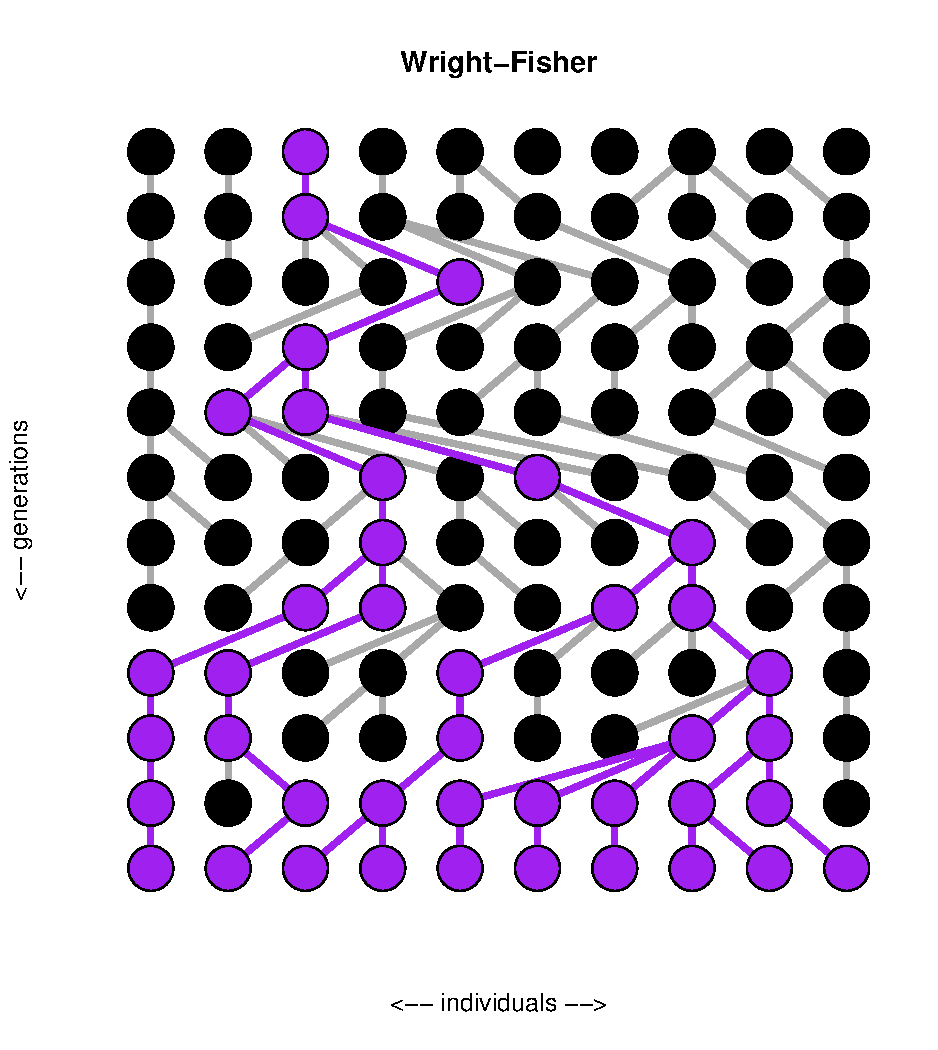
\includegraphics[width=0.5\textwidth]{eg_WF.pdf}\label{fig:eg_WF}}
\subfloat[][]{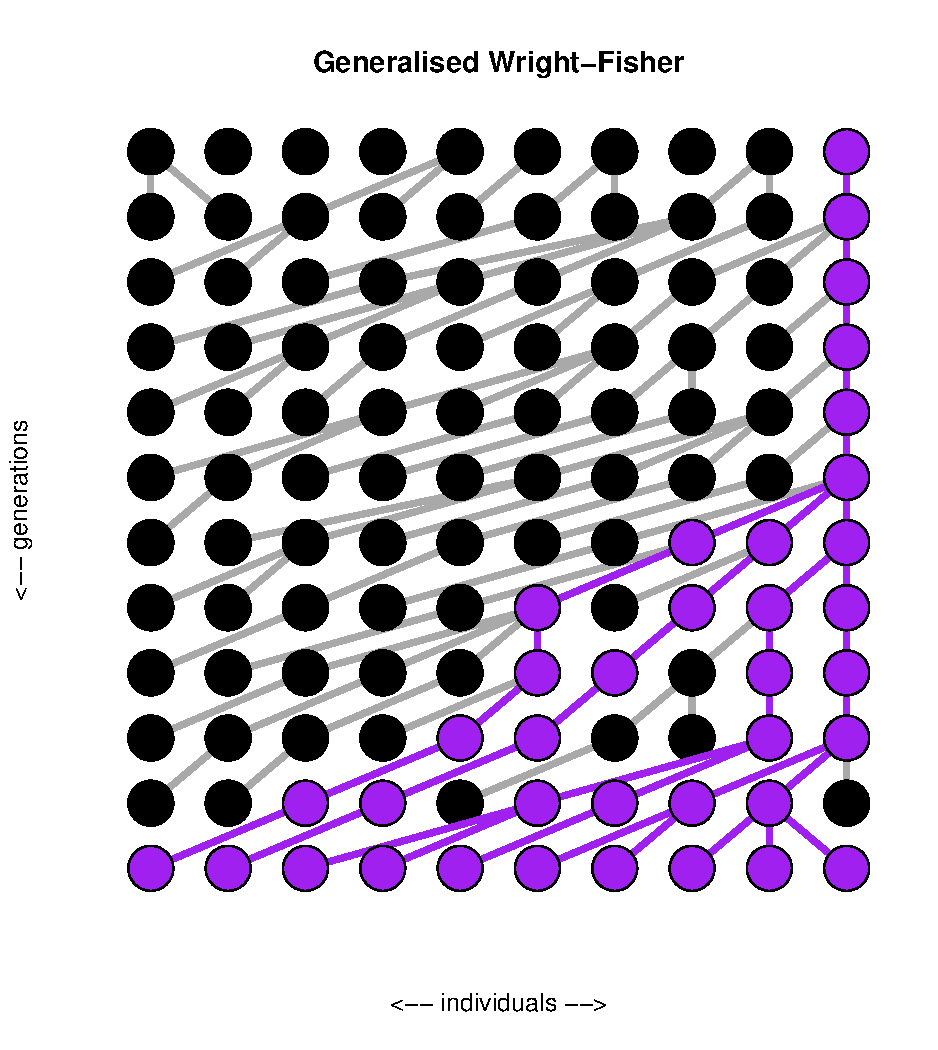
\includegraphics[width=0.5\textwidth]{eg_genWF.pdf}\label{fig:eg_genWF}}
\caption{Realisations from a Wright-Fisher model with $N=10$ individuals and 12 generations. (a) is from the standard model with uniform sampling probabilities. (b) is from the generalised model where individual $i$ is sampled with probability proportional to $i$. In both cases, the lineages of all the particles in the last generation are highlighted in order to give an impression of the coalescence mechanisms.}
\end{figure}

\subsubsection{Kingman's $n$-coalescent}
\citet{kingman1982gene} introduces the \emph{$n$-coalescent} as the asymptotic genealogical process for several population models, including the Wright-Fisher model, as the population size $N\to\infty$.
In the notation of \citet{wakeley2009}, let $T_i;\, i=2,\dots,n$ be the $i^{th}$ coalescence time, that is, the length of time for which there are exactly $i$ branches in the sample genealogy. The $n$-coalescent is the process in which these times are distributed as independent Exponentials:
\begin{equation*}
T_i \sim \operatorname{Exp}\left(\binom{i}{2}\right)
\end{equation*}
thus having
\begin{equation*}
\E(T_i) = \frac{2}{i(i-1)}, \qquad \V(T_i) = \left( \frac{2}{i(i-1)} \right)^2.
\end{equation*}
By noting that the number of possible pairs from $i$ lineages is $\frac{i(i-1)}{2}$, the process can be equivalently formulated as a Poisson process where pairs of lineages coalesce independently at rate 1, with the pair to coalesce being chosen uniformly at random \citep[Section 3.2]{wakeley2009}.
\citet{mohle1998} writes the same process in terms of the infinitesimal generator $Q$ of a Markov process on the set of equivalence relations on $n$ elements, having entries
\begin{equation*}
q_{\xi\eta} =
\begin{cases}
-\frac{1}{2}b(b-1) &\text{if }\xi=\eta \\
1 & \text{if }\xi \prec\eta \\
0 & \text{otherwise}
\end{cases}
\end{equation*}
where $b$ is the number of equivalence classes of $\xi$, and $\xi \prec \eta$ means that $\eta$ is a state with exactly one more pair of lineages coalesced compared to $\xi$.
 
\subsubsection{Application to SMC genealogies}
The Wright-Fisher model includes some simplifying assumptions that make it somewhat unrealistic for modelling populations (although they do not prevent it being useful in that context). Namely, it is assumed that the population size is constant, and that generations do not overlap. 
Gratifyingly, when the model is re-purposed for the analysis of SMC genealogies, both of these rather restrictive assumptions apply automatically. At least in the most common SMC algorithms, the number of particles (population size) remains constant at each iteration, and the resampling (reproduction) procedure is applied to all particles at once.

However, the standard Wright-Fisher model does not apply to SMC. The offspring distributions of each particle in a generation are not exchangeable, because broadly speaking, offspring of parents with high weight will tend to have high weight themselves. This follows intuitively from the notion that propagating a particle from a high density region at time $t$ will result in a new state that is close to the high density region at time $t+1$.

Some generalisations of the Wright-Fisher model were mentioned in Section \ref{sec:wf_models} that do not require exchangeability among individuals. But to model SMC genealogies it is necessary to go one step further, allowing dependence between the offspring distributions of different generations. This alteration amounts to a significant qualitative change since, while the forward process remains Markovian, the reverse (coalescent) process is no longer Markovian.

Whilst the population genetics literature has typically focused on the proliferation of hereditary traits \citep[Chapter 3]{wakeley2009}, our interest lies only with the genealogical process itself. The only ``traits'' of particles in SMC are their positions, and these are taken care of in the construction of the SMC algorithm (since it is deisrable to have many particles in high density regions). 
On the other hand, it is well-known that the problem of ``ancestral degeneracy'' is the source of much pain for practitioners; hence our interest in SMC genealogies themselves.

\subsection{Previous work}\label{sec:previous}
Kingman \citep{kingman1982gene, kingman1982coal, kingman1982exch} studied the asymptotic properties of the genealogies arising in a number of exchangeable population models, including the standard Wright-Fisher model. He showed that they each converge in the limit $N\to\infty$ (with appropriate time rescaling) to the $n$-coalescent. By studying this limiting process, he was able to establish some new results about the behaviour of such populations, and produce novel derivations of some known results.

\citet{mohle1998} extends this result to a class of non-exchangeable models, with the assumption that offspring distributions are independent between different generations. This allows application to more complex population models, such as the nest site model; but is still too restrictive to cover SMC genealogies, which by construction have strong dependence between generations.

Allowing for dependence between generations significantly complicates the computations, because the coalescent process is no longer Markovian. \citet{koskela2018} addresses a first case of such models, applicable to a range of standard SMC procedures, under some reasonable conditions.

We would like to extend to the case of conditional SMC, which differs substantially from the case of \citet{koskela2018} because there is a particular ancestral line that is conditioned to survive. This case would cover the particle Gibbs algorithm \citep{andrieu2010}, which is widely used in applications.

\subsubsection{Some details from the proofs}
The proofs of \citet{mohle1998} and \citet{koskela2018}, and ours by extension, rely on a decomposition of transitions into four cases.
Let $N$ be the constant population size, $v_i^{(r)}$ the (random) number of offspring in generation $r+1$ of individual $i$ in generation $r$, and let $\mathcal{R}_r$ be the equivalence relation that contains the pair $(i,j)$ iff individuals $i$ and $j$ in the final generation have a common ancestor in generation $r$. 
Note that in order to maintain a constant population size the offspring numbers must satisfy
\begin{equation}\label{eq:sum_vi}
\sum_{i=1}^{N} v_i^{(r)} = N.
\end{equation}
for all $r$.
Since particles cannot separate once coalesced, it is clear that $\{\mathcal{R}_r\}_{r \in \mathbb{N}}$ is a nested sequence of relations.
We use $\xi$ and $\eta$ to denote realisations of these relations, and consider now the possible one-step transitions.

Let $p_{\xi\eta}(r) := \PR(\mathcal{R}_r=\eta\mid\mathcal{R}_{r-1}=\xi)$ be the one-step transition probability. Due to the nesting of $\{\mathcal{R}_r\}_{r \in \mathbb{N}}$, this probability is non-zero only when $\xi \subseteq \eta$. That is, either $\eta=\xi$ or $\eta$ is obtained from $\xi$ by merging some lineages.
Let $\eta$ have $a$ equivalence classes, and let $\xi$ have $b = b_1 + \dots + b_a$ equivalence classes, where $b_i$ is the number of equivalence classes in $\xi$ that merge to become class $i$ in $\eta$.

A combinatorial argument allows us to derive an expression for the transition probability $p_{\xi\eta}(r)$ of the ancestral process:
\begin{equation}\label{eq:trans_prob}
p_{\xi\eta}(r) = \frac{1}{(N)_b} \sum_{\substack{i_1,\dots,i_a =1 \\ \text{distinct}}}^{N} \E\left[(v_{i_1}^{(r)})_{b_1}\cdots (v_{i_a}^{(r)})_{b_a}\right]
\end{equation}
The sum is over all the possible ordered choices of the $a$ parents from generation $r$. Inside the sum is the expected number of ways to have at least the required number of offspring from each parent, given this choice of parents. Thus the whole sum represents the probability of finding a set of parents that produce the required number of offspring. Then dividing by the number of ordered ways to choose $b$ offspring from generation $r-1$ ensures that the parents produce the \emph{correct} ordered offspring. Overall then we have the probability that exactly the right subsets of offspring from generation $r-1$ coalesce in generation $r$, counting all the different parents to which they could coalesce.

We define the the \emph{coalescence probability}, i.e.\ the probability that a randomly chosen pair of (distinct) individuals from generation $r-1$ have a common ancestor in generation $r$:
\begin{equation}
c_r := \frac{1}{(N)_2} \sum_{i=1}^{N} \E \left[ (v_i^{(r)})_2 \right] \label{eq:coal_prob1}
\end{equation}

We now reproduce the theorem given in \citet[Theorem 1]{mohle1998}, along with the first part of the proof, which also forms Lemma 1 of \citet{koskela2018}.
The proof will refer to the following identities and inequalities: \eqref{eq:tools_swap_sum_prod} is obtained using a multinomial expansion, \eqref{eq:tools_bernoulli_ineq} using Bernoulli's inequality, and \eqref{eq:tools_power_v_fact}--\eqref{eq:tools_fact_asymp2} by expanding factorials. 
\begin{align}
& \sum_{i_1\dots i_m = 1}^n \prod_{j=1}^m x_{i_j} = \prod_{j=1}^m \sum_{i=1}^n x_i = \left( \sum_{i=1}^n x_i \right)^m \label{eq:tools_swap_sum_prod}\\
& (k-x)^n = k^n\left(1-\frac{x}{k}\right)^n \leq k^n - nxk^{n-1} \label{eq:tools_bernoulli_ineq}\\
& n^a \geq (n)_a \label{eq:tools_power_v_fact}\\
%& (n)_a = (n)_b (n-b)_{a-b} \text{, if } 0\leq b\leq a \label{eq:tools_fact_take_two}\\
& (n)_a \leq (n)_b \,n^{a-b} \text{, if } 0\leq b\leq a \label{eq:tools_fact_taketwo_bd}\\
& \frac{n^{a-b}}{(n)_a} = \frac{1}{(n)_b} + O(n^{-b-1}) \label{eq:tools_fact_asymp1}\\
& \frac{1}{(n)_b} = \frac{1}{n^b} + O(n^{-b-1}) \label{eq:tools_fact_asymp2}
\end{align}

\begin{thm}\label{thm:mohle1}
Let $T \subset \mathbb{R}$ and suppose there is a function $\tau : T \to \mathbb{N}_0$ satisfying:
\begin{enumerate}[label=(\Alph*)]
\item\label{assn:coal_rate} correct limiting coalescence rate
\begin{equation*}
\forall t \in T, \,\lim_{N\to\infty} \sum_{r=1}^{\tau(t)} c_r =t
\end{equation*}
\item\label{assn:coal_var} variance of coalescence rate goes to zero
\begin{equation*}
\forall t \in T, \,\lim_{N\to\infty} \sum_{r=1}^{\tau(t)} c_r^2 =0
\end{equation*}
\item\label{assn:triple_coal} no triple coalescences
\begin{equation*}
\forall t \in T, \forall k\in\mathbb{N}_0,\, \lim_{N\to\infty} \sup_{r\leq\tau(t)} \frac{1}{N^3 c_r} \sum_{i=1}^N \E\left[ (v_i^{(r)})_2 (v_i^{(r)})^k \right] =0
\end{equation*}
\item\label{assn:multi_coal} only one coalescence at a time
\begin{equation*}
\forall t \in T,\, \lim_{N\to\infty} \sup_{r\leq\tau(t)} \frac{1}{N^4 c_r} \sum_{i,j=1}^N \E\left[ (v_i^{(r)})_2 (v_j^{(r)})^2 \right] =0
\end{equation*}
\end{enumerate}
Then the finite-dimensional distributions of $\{\mathcal{R}_{\tau(t)}\}_{t\in T}$ converge to those of the $n$-coalescent (with time restricted to $T$) in the limit $N\to\infty$.
\end{thm}
Note that, since $c_r \geq 0$ for all $r$, if \ref{assn:coal_rate} is assumed then \ref{assn:coal_var} is equivalent to
\begin{equation*}
\forall t \in T,\, \lim_{N\to\infty} \sup_{r\leq\tau(t)} c_r =0.
\end{equation*}

\begin{proof}
We first bound the transition probability $p_{\xi\eta}(r)$ as given by \eqref{eq:trans_prob}, in each of four possible cases. This will show that the only type of coalescence event to occur at any one time in the limit $N\to\infty$ is a merger of exactly one pair of lineages (\ref{case:pair_merge} below). 
We assume the offspring numbers $v_i^{(r)}$ are known (so we drop the expectations).
\begin{enumerate}[label = \textbf{Case \arabic*.}]
\item\label{case:pair_merge} $\eta$ is obtained from $\xi$ by merging exactly one pair of lineages, i.e.\ $b_1=2, b_2=\dots=b_a=1$, and $b=a+1$. We derive an upper bound:
\begin{align}
p_{\xi\eta}(r) &= \frac{1}{(N)_b} \sum_{\substack{i_1,\dots,i_a =1 \\ \text{distinct}}}^{N} (v_{i_1}^{(r)})_2(v_{i_2}^{(r)})_1\cdots (v_{i_a}^{(r)})_1 &\notag\\
&\leq \frac{1}{(N)_b} \sum_{i_1,\dots,i_a=1}^N (v_{i_1}^{(r)})_2 (v_{i_2}^{(r)})_1 \cdots (v_{i_a}^{(r)})_1 &\text{dropping distinctness} \notag\\
&= \frac{1}{(N)_b} \sum_{i=1}^N (v_i^{(r)})_2 \sum_{i_2,\dots,i_a=1}^N v_{i_2}^{(r)} \cdots v_{i_a}^{(r)} & \notag\\
&= \frac{1}{(N)_b} \sum_{i=1}^N (v_i^{(r)})_2 (v_1^{(r)} + \dots + v_N^{(r)})^{a-1} & \text{using \eqref{eq:tools_swap_sum_prod}} \notag\\
&= \frac{N^{b-2}}{(N)_b} \sum_{i=1}^N (v_i^{(r)})_2 & \text{using \eqref{eq:sum_vi}} \notag\\
&= \left( \frac{1}{(N)_2} + O(N^{-3}) \right) \sum_{i=1}^N (v_i^{(r)})_2 & \text{using \eqref{eq:tools_fact_asymp1}} \notag\\
&= c_r + o(c_r) & \text{by \eqref{eq:coal_prob1} and \ref{assn:triple_coal}} \notag
\end{align}
and a lower bound:
\begin{align}
p_{\xi\eta}(r) &= \frac{1}{(N)_b} \sum_{\substack{i_1,\dots,i_a =1 \\ \text{distinct}}}^{N} (v_{i_1}^{(r)})_2(v_{i_2}^{(r)})_1\cdots (v_{i_a}^{(r)})_1 &\notag\\
&= \frac{1}{(N)_b} \sum_{i=1}^N (v_i^{(r)})_2 \sum_{\substack{i_2,\dots,i_a =1 \\ \text{distinct} \neq i }}^{N} (v_{i_2}^{(r)})_1\cdots (v_{i_a}^{(r)})_1 &\notag\\
&\geq \frac{1}{(N)_b} \sum_{i=1}^N (v_i^{(r)})_2 \sum_{j\neq i} \sum_{\substack{i_3,\dots,i_a\\ \neq i}}\left[ v_j\cdot v_{i_3}\cdots v_{i_a} - \binom{b-2}{2}(v_j^{(r)})^2 \cdot v_{i_4}\cdots v_{i_a} \right] & \label{eq:transprob_lowerbd}\\
&= \frac{1}{(N)_b} \sum_{i=1}^N (v_i^{(r)})_2 \left[ \sum_{i_2,\dots,i_a\neq i} v_{i_2}\cdots v_{i_a} - \binom{b-2}{2} \sum_{i_3,\dots,i_a\neq i} v_{i_3}\cdots v_{i_a} \sum_{j \neq i} (v_j^{(r)})^2 \right] & \notag\\
&= \frac{1}{(N)_b} \sum_{i=1}^N (v_i^{(r)})_2 \left[ (N-v_i)^{b-2} - \binom{b-2}{2} \sum_{j\neq i} (v_j^{(r)})^2 N^{b-4} \right] &\text{using \eqref{eq:tools_swap_sum_prod}} \notag\\
&= \frac{1}{(N)_b} \sum_{i=1}^N (v_i^{(r)})_2  (N-v_i)^{b-2} - \frac{1}{(N)_b} \binom{b-2}{2} \sum_{i\neq j=1}^{N} (v_i^{(r)})_2 (v_j^{(r)})^2 N^{b-4} & \notag\\
&\geq \frac{1}{(N)_b} \sum_{i=1}^N (v_i^{(r)})_2  (N)^{b-2} - \frac{1}{(N)_b}(b-2)\sum_{i=1}^{N} (v_i^{(r)})_2 v_i^{(r)} N^{b-3} \notag\\
&\phantom{=\qquad\qquad} - \frac{1}{(N)_b}\binom{b-2}{2} \sum_{i\neq j=1}^{N} (v_i^{(r)})_2 (v_j^{(r)})^2 N^{b-4} &\text{using \eqref{eq:tools_bernoulli_ineq}} \notag\\
&\geq \frac{1}{(N)_2} \sum_{i=1}^N (v_i^{(r)})_2 - \frac{(b-2)N^{b-3}}{(N)_b}\sum_{i=1}^{N} (v_i^{(r)})_2 v_i^{(r)} \notag\\
&\phantom{=\qquad\qquad} -\frac{N^{b-4}}{(N)_b}\binom{b-2}{2} \sum_{i\neq j=1}^{N} (v_i^{(r)})_2 (v_j^{(r)})^2 & \notag\\
&= \frac{1}{(N)_2} \sum_{i=1}^N (v_i^{(r)})_2 - \left[\frac{(b-2)}{N^3} +O(N^{-4}) \right] \sum_{i=1}^{N} (v_i^{(r)})_2 v_i^{(r)} \notag\\
&\phantom{=\qquad\qquad} -\left[ \frac{1}{N^4}\binom{b-2}{2} + O(N^{-5}) \right] \sum_{i\neq j=1}^{N} (v_i^{(r)})_2 (v_j^{(r)})^2 &\text{using \eqref{eq:tools_fact_asymp1}, \eqref{eq:tools_fact_asymp2}} \notag\\
&= c_r + o(c_r) &\text{by \eqref{eq:coal_prob1},\ref{assn:triple_coal},\ref{assn:multi_coal}} \notag
\end{align}
Hence in this case $p_{\xi\eta}(r)=c_r +o(c_r)$.
The inequality \eqref{eq:transprob_lowerbd} is obtained by bounding the number of configurations with distinct parents by the the number of configurations with not necessarily distinct parents minus the number with at least one pair of parents chosen indistinctly. This leaves us with only the distinct-parents configurations since all indistinct choices must necessarily have a pair of parents chosen indistinctly, and the inequality arises from possible double-counting.

\item\label{case:triple_merge} $\eta$ is obtained from $\xi$ by merging three or more lineages into one, possibly along with other simultaneous mergers, i.e.\ $b_1\geq3$.
\begin{align}
p_{\xi\eta}(r) &= \frac{1}{(N)_b} \sum_{\substack{i_1,\dots,i_a =1 \\ \text{distinct}}}^{N} (v_{i_1}^{(r)})_{b_1}(v_{i_2}^{(r)})_{b_2}\cdots (v_{i_a}^{(r)})_{b_a} &\notag\\
&\leq \frac{1}{(N)_b} \sum_{i=1}^{N} (v_{i}^{(r)})_{b_1} \sum_{i_2,\dots,i_a =1}^{N} (v_{i_2}^{(r)})_{b_2}\cdots (v_{i_a}^{(r)})_{b_a} &\notag\\
&\leq \frac{1}{(N)_b} \sum_{i=1}^{N} (v_{i}^{(r)})_{b_1} (v_1^{(r)}+\dots+v_a^{(r)})^{b_2+\dots+b_a} &\text{using \eqref{eq:tools_swap_sum_prod}} \notag\\
&\leq \frac{1}{(N)_b} \sum_{i=1}^{N} (v_{i}^{(r)})_{b_1} N^{b-3} &\text{since }b_2+\dots+b_a\leq b-3 \label{eq:triplemerge_bound_spinoff}\\
&\leq \frac{N^{b-3}}{(N)_b} \sum_{i=1}^{N} (v_{i}^{(r)})_{2}(v_{i}^{(r)})^{b_1-2}  &\text{using \eqref{eq:tools_fact_taketwo_bd}} \notag\\
&= o(c_r) &\text{using \ref{assn:triple_coal}} \notag
\end{align}

\item\label{case:multi_merge} $\eta$ is obtained from $\xi$ via two or more pair mergers, with no mergers of more than two lineages, i.e.\ $2=b_1=b_2\geq b_3\geq\dots\geq b_a\geq1$.
\begin{align}
p_{\xi\eta}(r) &= \frac{1}{(N)_b} \sum_{\substack{i_1,\dots,i_a =1 \\ \text{distinct}}}^{N} (v_{i_1}^{(r)})_2 (v_{i_2}^{(r)})_2 (v_{i_3}^{(r)})_{b_3}\cdots (v_{i_a}^{(r)})_{b_a} &\notag\\
&\leq \frac{1}{(N)_b} \sum_{i=1}^{N} (v_{i}^{(r)})_2 \sum_{j=1}^N (v_j^{(r)})_2 \sum_{i_3,\dots,i_a =1}^{N} (v_{i_3}^{(r)})_{b_3}\cdots (v_{i_a}^{(r)})_{b_a} &\text{dropping distinctness}\notag\\
&\leq \frac{1}{(N)_b} \sum_{i=1}^{N} (v_{i}^{(r)})_2 \sum_{j=1}^N (v_j^{(r)})^2 \sum_{i_3,\dots,i_a =1}^{N} (v_{i_3}^{(r)})_{b_3}\cdots (v_{i_a}^{(r)})_{b_a} &\text{using \eqref{eq:tools_power_v_fact}} \notag\\
&\leq \frac{1}{(N)_b} \sum_{i,j=1}^{N} (v_{i}^{(r)})_2 (v_j^{(r)})^2 (v_1^{(r)}+\dots+v_N^{(r)})^{b_3+\dots +b_a} &\notag\\
&=\frac{N^{b-4}}{(N)_b} \sum_{i,j=1}^N (v_{i}^{(r)})_2 (v_j^{(r)})^2 & \\
&= o(c_r) &\text{using \ref{assn:multi_coal}} \notag
\end{align}

\item\label{case:no_change} No mergers occur: $\eta=\xi$, i.e.\ $b_1=\dots=b_a=1$, and $a=b$.
\begin{align}
p_{\xi\xi}(r) &= \frac{1}{(N)_a} \sum_{\substack{i_1,\dots,i_a =1 \\ \text{distinct}}}^{N} (v_{i_1}^{(r)})_1  \cdots (v_{i_a}^{(r)})_1 & \notag\\
&= \frac{1}{(N)_a} \sum_{\substack{i_1,\dots,i_a =1 \\ \text{distinct}}}^{N} v_{i_1}^{(r)} \cdots v_{i_a}^{(r)} & \notag\\
&= \frac{1}{(N)_a} \left[ \sum_{i_1,\dots,i_a =1}^N v_{i_1}^{(r)} \cdots v_{i_a}^{(r)} - \binom{a}{2}\sum_{j=1}^N (v_j^{(r)})^2 \sum_{i_3,\dots,i_a =1}^N v_{i_3}^{(r)} \cdots v_{i_a}^{(r)} \right] &\label{eq:transprob_lowerbd2}\\
&= \frac{1}{(N)_a} \left[ (v_1^{(r)}+\dots+v_N^{(r)})^a - \binom{a}{2} \sum_{i=1}^N (v_i^{(r)})^2 (v_1^{(r)}+\dots+v_N^{(r)})^{a-2} \right] &\text{using \eqref{eq:tools_swap_sum_prod}} \notag\\
&= \frac{1}{(N)_a} \left[ N^a - \binom{a}{2} N^{a-2} \sum_{i=1}^N (v_i^{(r)})^2 \right] &\notag\\
&\geq 1- \binom{a}{2} \frac{N^{a-2}}{(N)_a} \sum_{i=1}^N (v_i^{(r)})^2 &\text{using \eqref{eq:tools_power_v_fact}}\notag\\
%&= 1- \binom{a}{2} \frac{N^{a-2}}{(N)_2 (N-2)_{a-2}} \sum_{i=1}^N (v_i^{(r)})^2 &\text{using \eqref{eq:tools_fact_take_two}}\notag\\
&= 1- \binom{a}{2} \left[ \frac{1}{(N)_2} + O(N^{-3}) \right] \sum_{i=1}^N (v_i^{(r)})^2 &\text{using \eqref{eq:tools_fact_asymp1}}\\
&= 1- c_r +o(c_r) &\notag
\end{align}
\end{enumerate}
The equality \eqref{eq:transprob_lowerbd2} is obtained in the same way as \eqref{eq:transprob_lowerbd}, with no double-counting.
We have now shown that the only coalescence events having positive probability in the limit $N\to\infty$ are staying the same (\ref{case:no_change}) or merging a single pair of lineages (\ref{case:pair_merge}). All other possibilities have asymptotic probability $o(c_r)$.

To complete the proof of Theorem \ref{thm:mohle1}, it remains to show that the finite-dimensional distributions of the genealogical process converge to those of the $n$-coalescent. Because the processes considered are Markov even backwards in time, it suffices to show that the generators of the process converge to the generators of the Kingman coalescent, and this is how \citet{mohle1998} concludes the proof.
\end{proof}

For the argument of \citet{koskela2018}, a different form is needed for the upper bound on triple mergers (\ref{case:triple_merge}). Starting from \eqref{eq:triplemerge_bound_spinoff}, we obtain:
\begin{align}
p_{\xi\eta}(r) &\leq \frac{1}{(N)_b} \sum_{i=1}^{N} (v_{i}^{(r)})_{b_1} N^{b-3} \notag\\
&\leq \frac{N^{b-3}}{(N)_b} \sum_{i=1}^{N} (v_{i}^{(r)})^{b_1} \notag\\
&= \left[ \frac{1}{N^3} + O(N^{-4}) \right] \sum_{i=1}^{N} (v_{i}^{(r)})^{b_1}
\end{align}


\section{Theoretical results}\label{sec:theory}
In this section we present an extension of the results of \citet{koskela2018} to the case of conditional SMC, where a predetermined trajectory, the ``immortal line'', is conditioned to survive. The argument follows that of \citet{koskela2018}, with a few modifications.
We concentrate on the exchangeable model, so we may take without loss of generality that the immortal line is the trajectory containing individual 1 from each generation.
We first assume the simplest case, with multinomial resampling (see Algorithm \ref{alg:condSMC}). The analogous standard SMC algorithm has marginal offspring distributions
\begin{equation*}
\vt{i} \eqdist \Bin (N, \wt{i}), \qquad i=1,\dots,N
\end{equation*}
which yield the coalescence rate
\begin{equation}
c_N(t) := \frac{1}{(N)_2} \sum_{i=1}^{N} \E\left[ (\vt{i})_2 \right] = \sum_{i=1}^{N} \E\left[(\wt{i})^2\right].
\end{equation}
But now, to ensure the immortal line survives, individual 1 in each time step necessarily produces at least one offspring. It is straighforward to check that under this conditioning, the remaining $N-1$ offspring are assigned multinomially to the $N$ possible parents as usual. This leads to the following offspring distributions:
\begin{align*}
& \vttilde{1} \eqdist 1 + \Bin(N-1, \wt{1}) \\
& \vttilde{i} \eqdist \Bin(N-1, \wt{i}), \qquad i=2,\dots,N.
\end{align*}
We therefore have the following moments (using the tower property):
\begin{align*}
& \E[\vttilde{i}] = (N-1)\E[\wt{i}] &\\
& \E[(\vttilde{i})^2] = (N-1)(N-2)\E[(\wt{i})^2] + (N-1)\E[\wt{i}] &\qquad i=2,\dots,N \\
& \E[\vttilde{1}] = (N-1)\E[\wt{1}] + 1 \\
& \E[(\vttilde{1})^2] = (N-1)(N-2)\E[(\wt{1})^2] + 3(N-1)\E[\wt{1}] + 1 &
\end{align*}
and we can derive the altered coalescence rate:
\begin{align}
\tilde{c}_N(t) &= \frac{1}{(N)_2} \sum_{i=1}^{N} \E\left[ (\vttilde{i})_2 \right] \notag\\
&= \frac{1}{(N)_2} \E\left[ (\vttilde{1})^2 - \vttilde{1} \right] + \frac{1}{(N)_2}\sum_{i=2}^{N} \E\left[ (\vttilde{i})^2 - \vttilde{i} \right] \notag\\
&= \frac{1}{(N)_2}\left[ (N-1)(N-2)\E[(\wt{1})^2] + 2(N-1)\E[\wt{1}] \right] + \frac{1}{(N)_2} \sum_{i=2}^{N} (N-1)(N-2)\E[(\wt{i})^2] \notag\\
&= \frac{1}{(N)_2} \sum_{i=1}^{N} (N-1)(N-2)\E[(\wt{i})^2] + \frac{1}{(N)_2} 2(N-1)\E[\wt{1}] \notag\\
&= \frac{N-2}{N} c_N(t) + \frac{2}{N} \E[\wt{1}]
%&\overset{N\to\infty}{\longrightarrow} c_N(t) \notag
\end{align}
%Since $\wt{1} \leq 1$ for all $t$, as $N\to\infty$ we have
%\begin{equation*}
%\tilde{c}_N(t) - c_N(t) = O(N^{-1}).
%\end{equation*}
Under the conditions of \citet[Corollary 2]{koskela2018}, we have that $\E[\wt{1}] = O(N^{-1})$, and hence
\begin{equation*}
\tilde{c}_N(t) - c_N(t) = O(N^{-2}).
\end{equation*}
%\begin{equation*}
%\tilde{c}_N(t) = \frac{N-2}{N} c_N(t) + O(N^{-2}) = c_N(t) + O \left( \frac{c_N(t)}{N} \right)
%\end{equation*}
\citet{koskela2018} states the following bounds on $c_N(t)$:
\begin{equation*}
\frac{C_*}{N-1} \leq c_N(t) \leq \frac{C}{N-1}.
\end{equation*}
Since $\tilde{c}_N(t)$ differs from $c_N(t)$ by $O(N^{-2})$, for sufficiently large $N$ there exist constants $\tilde{C}, \tilde{C}_*$ such that
\begin{equation*}
\frac{\tilde{C}_*}{N-1} \leq \tilde{c}_N(t) \leq \frac{\tilde{C}}{N-1}
\end{equation*}
and we can thus derive bounds analogous to \citet[(5)-(6)]{koskela2018}:
\begin{align}
\frac{N-1}{\tilde{C}_*}t &\leq \tilde{\tau}_N(t) \leq \frac{N-1}{\tilde{C}}t \label{eq:tau_bounds1}\\
\frac{N-1}{\tilde{C}_*}(s-t) &\leq \tilde{\tau}_N(s) - \tilde{\tau}_N(t) \leq \frac{N-1}{\tilde{C}}(s-t) \label{eq:tau_bounds2}
\end{align}
Furthermore, we have that
\begin{align*}
\frac{\tilde{C}}{N-1} &= \frac{N-2}{N} \frac{C}{N-1} + O(N^{-2}) \\
&= \frac{C}{N-1} + O(N^{-2})
\end{align*}
therefore $\tilde{C} - C = O(N^{-1})$ and similarly $\tilde{C}_* - C_* = O(N^{-1})$. 
This means that the bounds \eqref{eq:tau_bounds1}, \eqref{eq:tau_bounds2} are asymptotically equal to \citet[(5)--(6)]{koskela2018}.

It remains to verify that the conditions \citep[(3)--(4)]{koskela2018} can extend to this case. If so, a modified version of \citet[Theorem 1]{koskela2018} and its corollaries will hold, by the same argument, for conditional SMC. This will be the next focus in our research on this topic.

\section{Simulation study}\label{sec:simulations}
In order to investigate how well the asymptotic results hold for finite $N$, we conducted a simulation study on the Ornstein-Uhlenbeck model, a ``simplest case'' hidden Markov model which is typical for empirical tests in the literature. The process is defined as follows:
\begin{align*}
& X_0 \sim \N(0,1) \\
& X_{t+1} \mid X_t \sim \N((1-\Delta)X_t, \Delta) \\
& Y_t \mid X_{t} \sim \N(X_t, \sigma^2)
\end{align*}
with parameters $\Delta >0, \sigma >0$.

Tree height $T$ is one of the basic properties of ancestral trees, and has a useful interpretation in the context of population genetics. It denotes the number of generations back one must go to find the most recent common ancestor (MRCA) of a sample of $n$ individiuals from generation $N_{obs}$ (leaves). That is, the number of steps of the reverse process that pass before the $n$ sampled lineages all coalesce to a single lineage. For the $n$-coalescent, moments of $T$ are available analytically. In particular, we expect conditional SMC to have the same limiting process as standard SMC, since we have shown in Section \ref{sec:theory} that their coalescent rates are asymptotically equal. Therefore in the limit as $N\to\infty$ we expect the moments of $T$ to behave as stated in \citet[Corollary 1]{koskela2018}:
\begin{align*}
\frac{C_*}{C^2} \left(1-\frac{1}{n}\right) + O(N^{-1}) &\leq \E[T/N] \leq 2\frac{C}{C_*^2} \left(1-\frac{1}{n}\right) \\
\left(\frac{4\pi^2}{3} - 12 + O(n^{-1})\right) \left(\frac{C_*}{C^2}\right)^2 + O(N^{-1}) &\leq \V(T/N) \leq \left(\frac{4\pi^2}{3} - 12 + O(n^{-1})\right) \left(\frac{C}{C_*^2}\right)^2
\end{align*}
where of course $T$ depends on $n$ and $N$. In particular, the choice of immortal line does not feature in these bounds and so should have no effect as $N \to\infty$ with respect to $n$.

Following \citet{koskela2018}, we take $\Delta = \sigma = 0.1$ and generate one fixed sequence of observations for use in all SMC runs.
We use a range of values $\{256, 512, \dots, 4096\}$ for $N$, and two fixed values $n=2,16$ intended to show the qualitative difference in behaviour as we cross a supposed ``$n<<N$'' threshold.
The number of observations $N_{obs}$ is taken such that, for all the choices of $n$ and $N$, the $N_{obs}$ generations of SMC particles are enough for the $n$ sampled lineages to coalesce to one common ancestor by generation 0 (with high enough probability that it happens reliably on every repetition), ensuring that the tree height can always be recorded.

For this toy model, the smoothing distribution is available analytically through the Rauch-Tung-Striebel (RTS) smoother \citep{rauch1965}. We exploit this solution to choose the ``immortal line'' on which to condition the conditional SMC updates. Because both the MAP estimate (which is equal to the mean since the distributions are Gaussian) and variance are available via the RTS smoother, we are able to produce a sequence of immortal lines of decreasing likelihood, by adding multiples of the standard deviation to the mean.

We hypothesise that when $N$ is not too much bigger than $n$, a more unlikely choice of the immortal line should produce qualitative differences in the tree height profile. If $n$ is large compared to $N$, the sampled lineages would be relatively likely to meet the immortal line, in which case they must also coalesce onto the immortal line. If the immortal line is close to the MAP then this is not particularly strange behaviour, but if the immortal line is an unlikely trajectory then this will corresponds to an unlikely choice of ancestors under the unconditional algorithm. 

As $N\to\infty$ with respect to $n$, the probability of the sampled lineages meeting the immortal line goes to 0, so this effect should become insignificant.

Figures \ref{fig:kalman_n16} and \ref{fig:kalman_n2} illustrate this distinction. Here we use a decrease in $n$ as a proxy for increasing $N$: over the same range of values for $N$, Figure \ref{fig:kalman_n16} shows the profile for sample size $n=16$, and Figure \ref{fig:kalman_n2} for $n=2$.
We see clearly that in the case $n=16$, the likelihood of the immortal line significantly affects the tree height profile, while for $n=2$ it makes no appreciable difference.

Figure \ref{fig:standardSMC} shows corresponding results for standard SMC. Comparing the $n=2$ line to Figure \ref{fig:kalman_n2}, it seems that the tree height is larger for conditional SMC than for standard SMC. We believe this effect should diminish asymptotically, but further investigation is required.

\begin{figure}
\centering
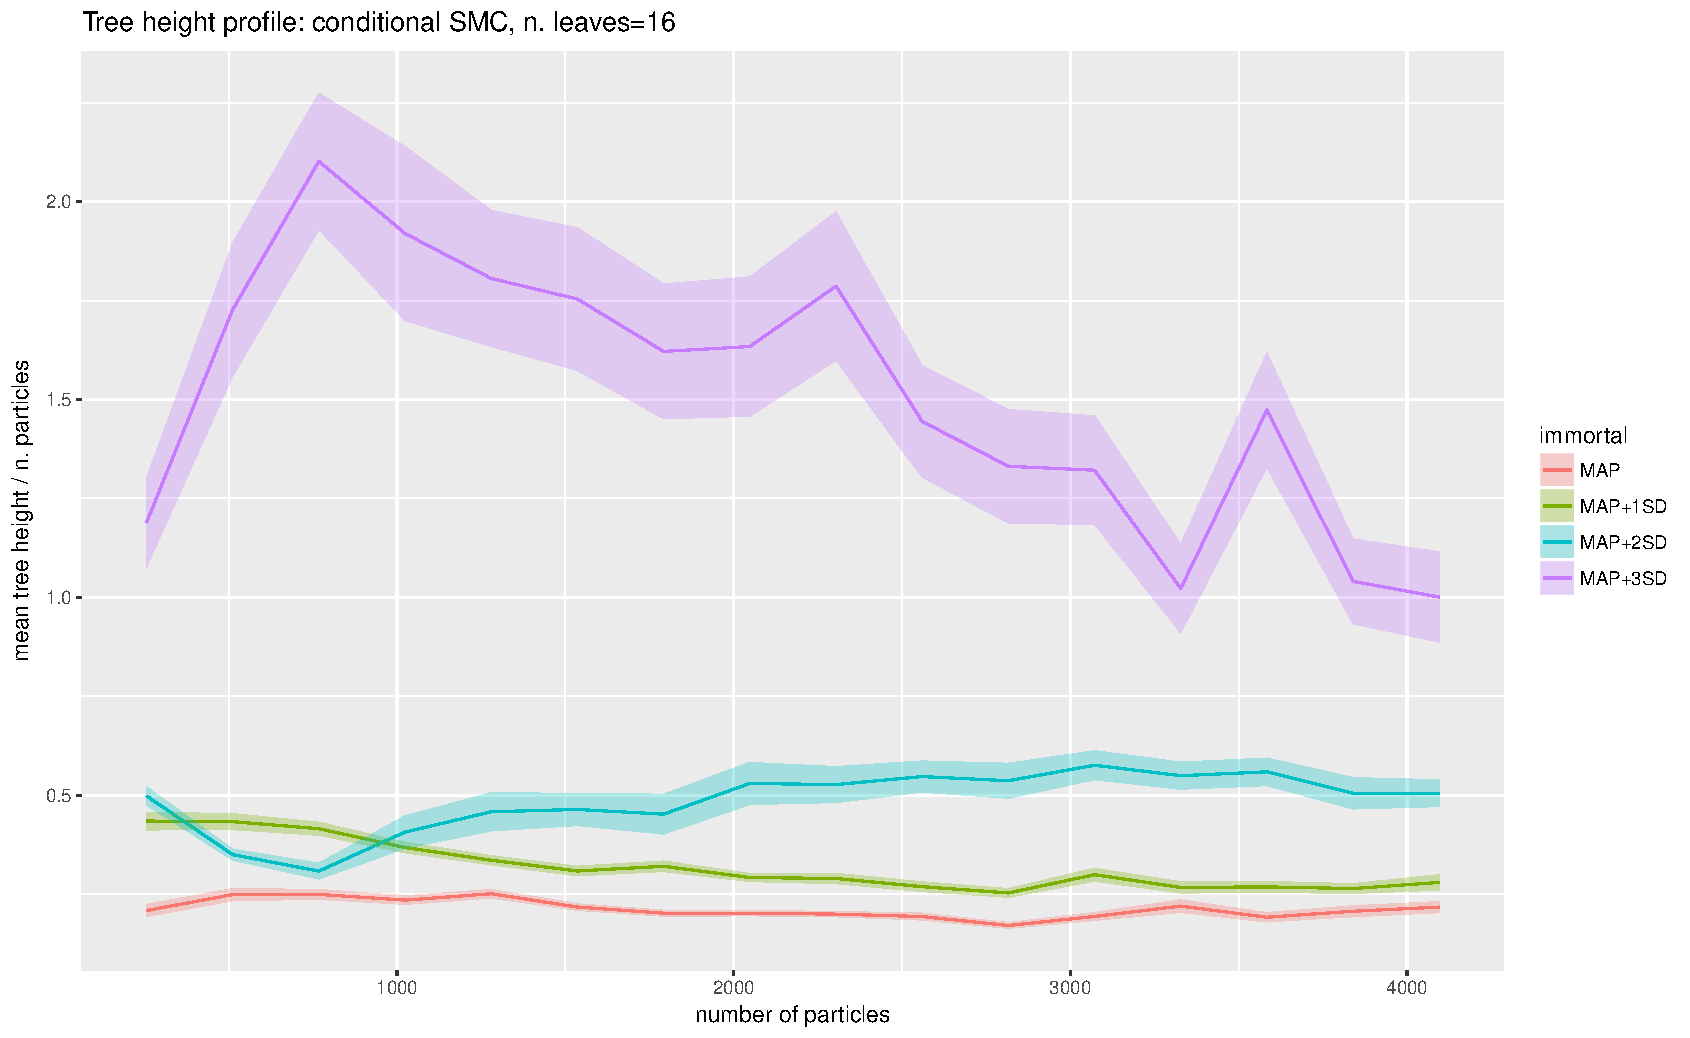
\includegraphics[width=\textwidth]{kalman_n16_100reps_line.pdf}
\caption{$\E(T/N)$ for samples of $n=16$ leaves from conditional SMC genealogies where the immortal line is taken to be 0,1,2,3 standard deviations away from the MAP estimate. Each point is averaged over 100 repetitions of running the particle filter and sampling $n$ leaves; and the same sequence of observations was used for every run. Here different choices of immortal line seem to have a profound effect on the mean tree height.}
\label{fig:kalman_n16}
\end{figure}
\begin{figure}
\centering
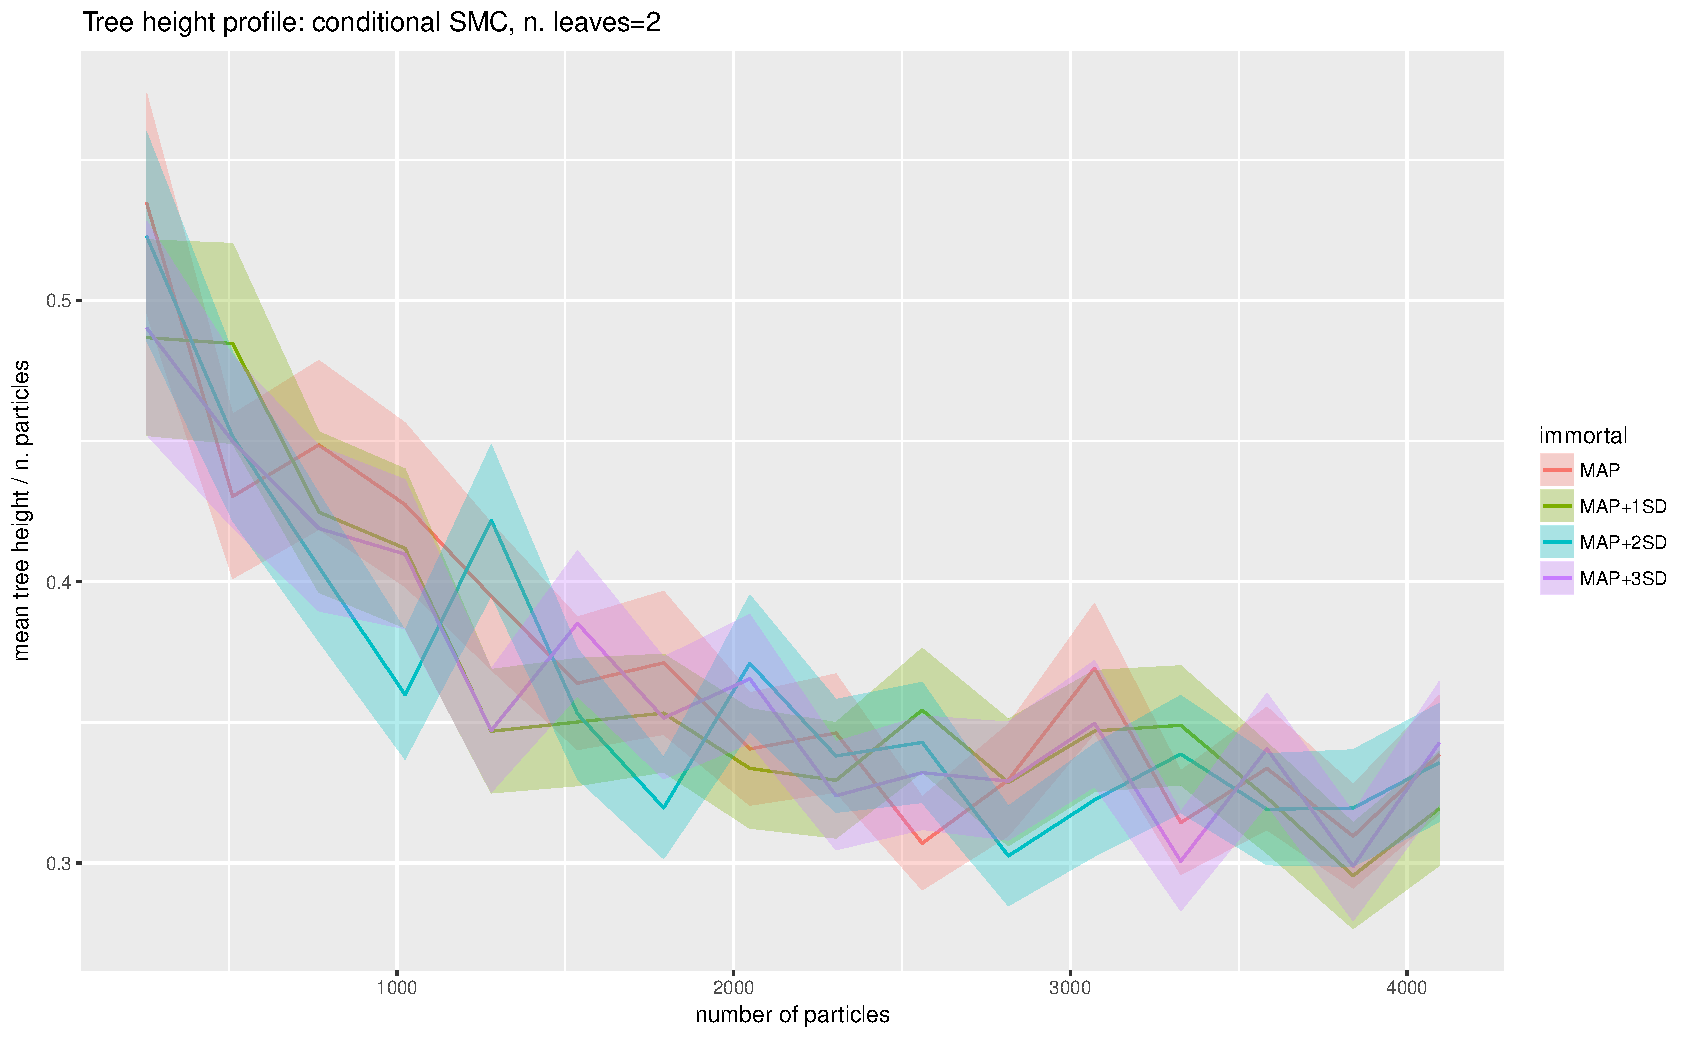
\includegraphics[width=\textwidth]{kalman_n2_1000reps_line.pdf}
\caption{$\E(T/N)$ for samples of $n=2$ leaves from conditional SMC genealogies where the immortal line is 0,1,2,3 standard deviations away from the MAP estimate. Each point is averaged over 1000 repetitions of running the particle filter and sampling $n$ leaves; and the same sequence of observations was used for every run. Here the choice of immortal line does not seem to affect the mean tree height.}
\label{fig:kalman_n2}
\end{figure}
\begin{figure}
\centering
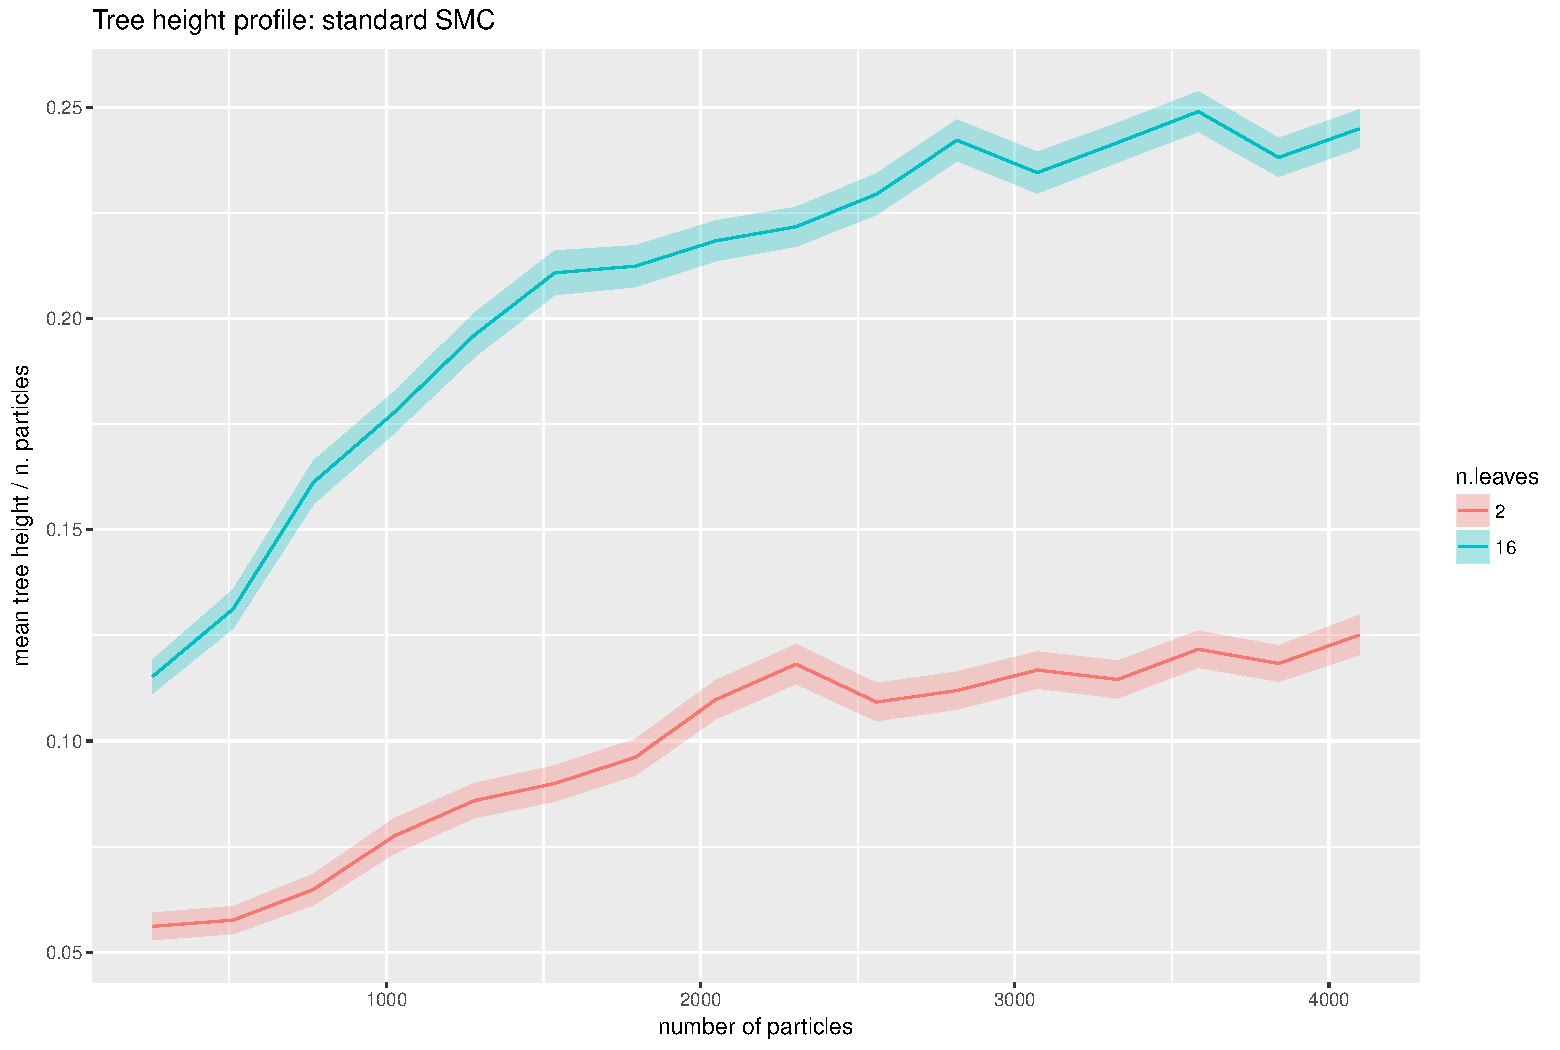
\includegraphics[width=0.9\textwidth]{treeht_std_1000reps.pdf}
\caption{$\E(T/N)$ for samples of $n=2$ and $n=16$ leaves from standard SMC genealogies. Each point is averaged over 1000 repetitions of running the particle filter and sampling $n$ leaves; and the same sequence of observations was used for every run.}
\label{fig:standardSMC}
\end{figure}

\section{Conclusions}
We have showed that under multinomial resampling, the coalescence probability for conditional SMC is close enough to that of standard SMC to imply the existence of a time rescaling that is asymptotically equivalent to that defined in \citet[p.7]{koskela2018}. Given this result, we expect the conclusions presented in \citet{koskela2018} to be transferable to the conditional SMC setting. However, conditions \citet[(3)--(4)]{koskela2018} still need to be verified before this can be made rigorous.

While \citet[Section 3]{koskela2018} demonstrates that in the case of standard SMC, the asymptotic results seem to hold even for $n=N$, we conclude from our simulation study that the results for conditional SMC only apply asymptotically. This is not surprising given the substantial qualitative differences between SMC and conditional SMC genealogies, which remain significant when $n$ is too close to $N$.

Although we have demonstrated empirically that $n <<N$ is required to mitigate the effect of choosing an unlikely immortal line, this in itself should not be of concern when the results are applied to particle Gibbs. In the particle Gibbs algorithm, an immortal line is sampled at each iteration from the trajectories generated in the previous iteration, proportionally to their likelihood. Unless all the generated trajectories are unlikely (in which case there are more profound problems with the algorithm), the immortal line will therefore tend to be a reasonably likely one.

We expect that less straight-forward conditional SMC algorithms, using alternative resampling schemes, should have the same limiting genealogical process (up to constants) as the multinomial scheme; as was hypothesised and demonstrated empirically in \citet{koskela2018} for standard SMC. However, proving this even for standard SMC remains an open problem.

There are many other directions for generalising these results, both theoretical and empirical, particularly investigating their robustness under violation of the various assumptions. It is of particular interest to consider the classes of SMC algorithms most commonly used in practice, and examine the compatibility of our assumptions with these applications.

\bibliography{smc.bib}
\end{document}